%%%%%%%%%%%%%%%%%%%%%%%%%%%%%%%%%%%%%%%%%%%%%%%%%%%
%
%  New template code for TAMU Theses and Dissertations starting Fall 2012.  
%  For more info about this template or the 
%  TAMU LaTeX User's Group, see http://www.howdy.me/.
%
%  Author: Wendy Lynn Turner 
%	 Version 1.0 
%  Last updated 8/5/2012
%
%%%%%%%%%%%%%%%%%%%%%%%%%%%%%%%%%%%%%%%%%%%%%%%%%%%
%%%                           APPENDIX - Chapter 3
%%%%%%%%%%%%%%%%%%%%%%%%%%%%%%%%%%%%%%%%%%%%%%%%%%%

\phantomsection
\chapter{\uppercase{Addendum to Section \ref{sec::BF}}}
\label{sec::appendix_BF}

%%%%%%%%%%%%%%%%%%%%%%%%%%%%%%%%%%%%%%%%%%%%%%%%%%%
%%%   Section - Limits of the Linear Polygonal Basis Functions
\section{Limits of the Linear Polygonal Basis Functions}
\label{sec::appendix_BF_Limits}

As it was stated in Chapter \ref{sec::B}, the Wachspress, mean value, and maximum entropy coordinates are all undefined on the boundary of the polygonal element. However, these basis functions do have a valid limit on the boundary. This means that while direct boundary evaluation of the coordinates is impossible (results in divide-by-zero issues), we can demonstrate that the limits of their values are exactly those required of general barycentric coordinates. We use the geometric properties for an arbitrary polygon presented in Figure \ref{fig::App_BF_2D_ref_polygon} to do this.

\begin{figure}
\centering
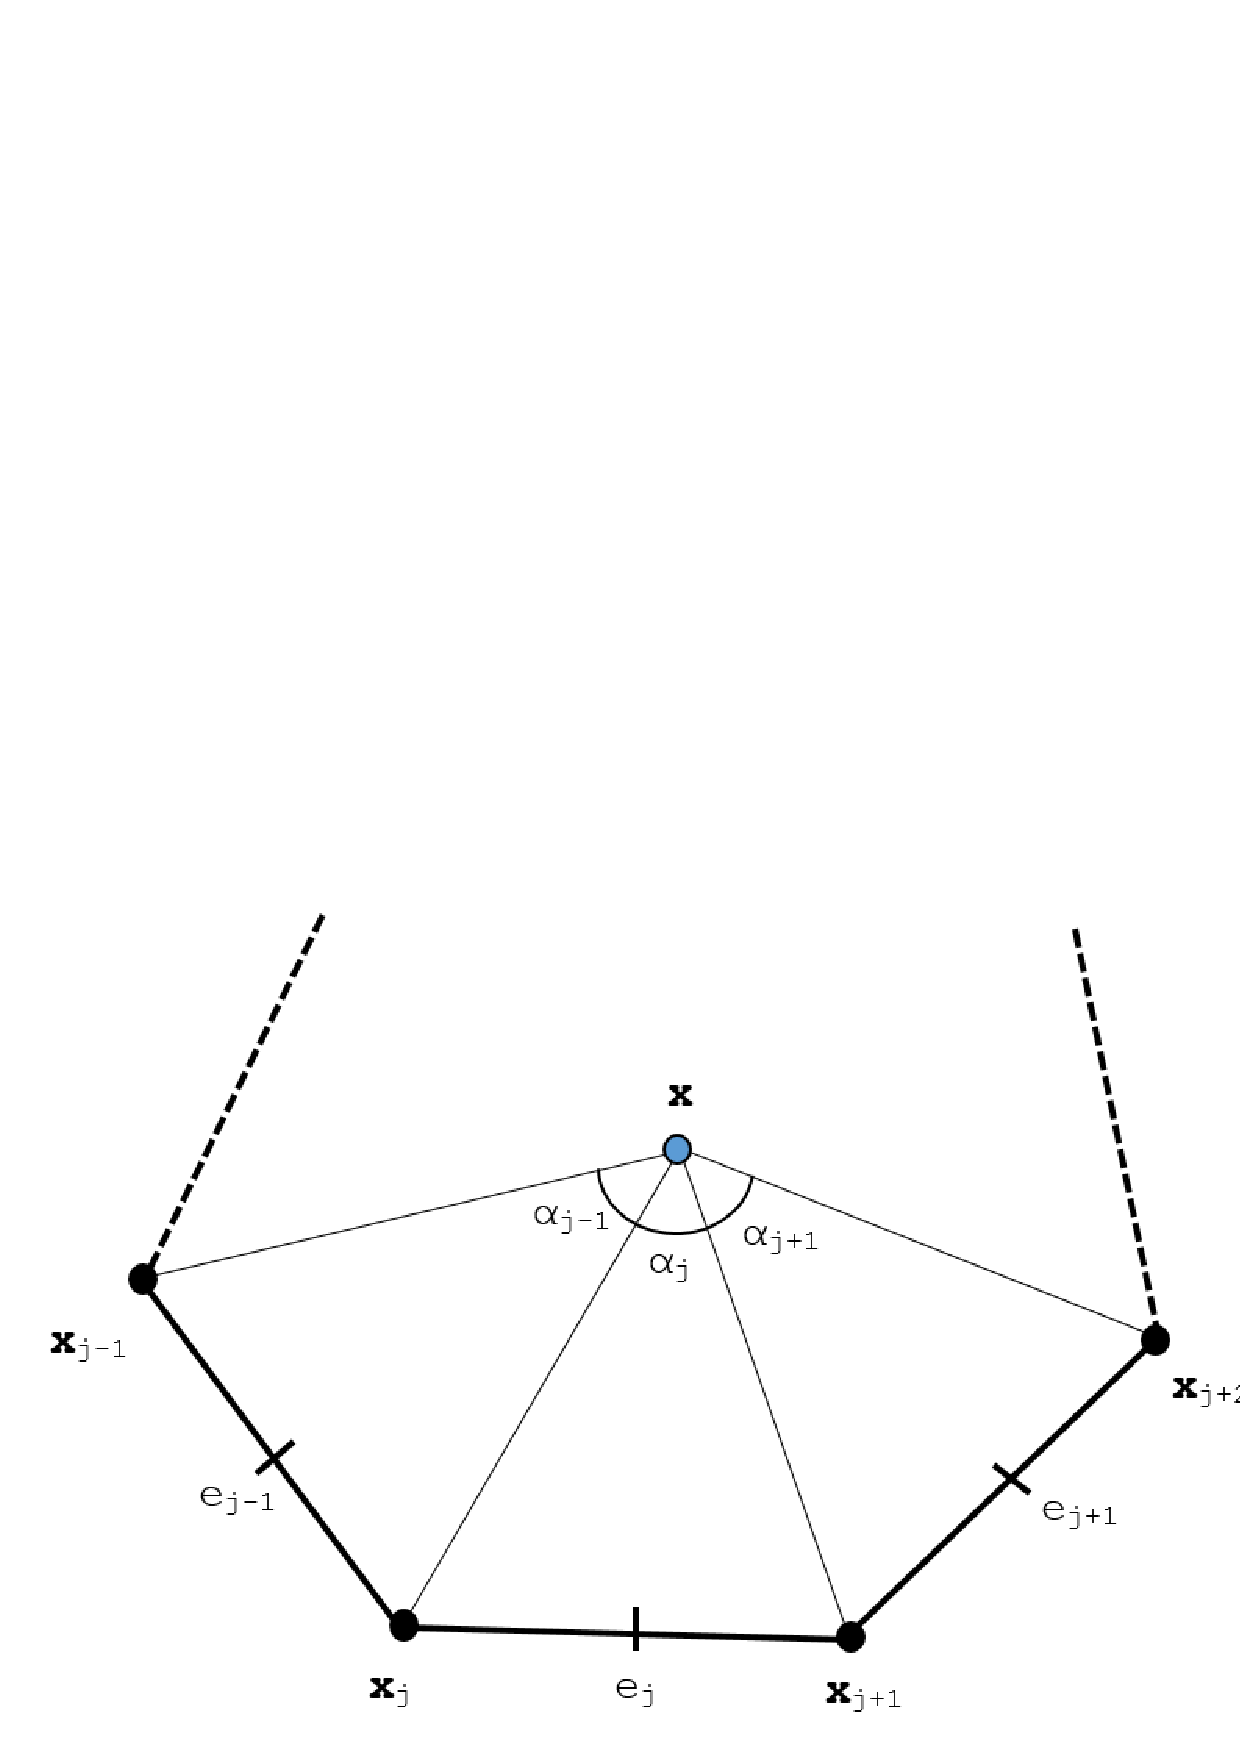
\includegraphics[width=0.65\textwidth]{figures/appendices/ref_polygon.png}
\caption{Arbitrary polygon with geometric properties used for 2D basis function generation.}
\label{fig::App_BF_2D_ref_polygon}
\end{figure}

%%%%%%%%%%%%%%%%%%%%%%%%%%%%%%%%%%%%%%%%%%%%%%%%%%%
%%%  Sub Section - Wachspress Limits
\subsection{Limits of the Wachspress Coordinates}
\label{sec::appendix_BF_Limits_Wachspress}

Recall from Section \ref{sec::BF_2DLinear_Wachspress} that the Wachspress basis functions are of the form

\begin{equation}
\label{eq::App_BF_WachBF}
\lambda_i (\vec{x}) = \frac{w_i^W  (\vec{x}) }{\sum_j w_j^W  (\vec{x}) },
\end{equation}

\noindent where the weight function for vertex $i$, $w_i$, has the following definition:

\begin{equation}
\label{eq::App_BF_wach_weights}
w_i (\vec{x})  = \frac{A(\vec{x}_{i-1}, \vec{x}_{i}, \vec{x}_{i+1})}{A(\vec{x}, \vec{x}_{i-1}, \vec{x}_{i}) \, A(\vec{x}, \vec{x}_{i}, \vec{x}_{i+1})} .
\end{equation}

First, we analyze the limiting case as the point of evaluation, $\vec{x}$, approaches a vertex. The Wachspress coordinates maintain the {\em Lagrange property}: $\lambda_i (\vec{x}_j)=\delta_{ij}$. We prove this now by first dividing the numerator and denominator of Eq. (\ref{eq::App_BF_WachBF}) through by $w_j$ to yield the following:

\begin{equation}
\label{eq::App_BF_wach_divide}
\lambda_i (\vec{x}) = \frac{w_i/w_j}{1+\sum_{k\neq j} w_k/w_j}, \, i \neq j \qquad \text{and} \qquad \lambda_j (\vec{x}) = \frac{1}{1+\sum_{k\neq j} w_k/w_j} .
\end{equation}

%%%%%%%%%%%%%%%%%%%%%%%%%%%%%%%%%%%%%%%%%%%%%%%%%%%
%%%  Sub Section - MV Limits
\subsection{Limits of the Mean Value Coordinates}
\label{sec::appendix_BF_Limits_MV}

Recall from Section \ref{sec::BF_2DLinear_MV} that the mean value basis functions are of the form

\begin{equation}
\label{eq::App_BF_MVBF}
\lambda_i (\vec{x}) = \frac{w_i^{MV}  (\vec{x}) }{\sum_j w_j^{MV}  (\vec{x}) }
\end{equation}

\noindent where the weight function for vertex $i$, $w_i$, has the following definition:

\begin{equation}
\label{eq::App_BF_MV_weights}
w_i (\vec{x})  = \frac{\tan(\alpha_{i-1} / 2) + \tan(\alpha_i / 2)}{|\vec{x}_i - \vec{x}|}
\end{equation}

First, we analyze the limiting case as the point of evaluation, $\vec{x}$, approaches a vertex. The mean value coordinates maintain the {\em Lagrange property}: $\lambda_i (\vec{x}_j)=\delta_{ij}$. We prove this now by first dividing the numerator and denominator of Eq. (\ref{eq::App_BF_MVBF}) through by $w_j$ to yield the following:

\begin{equation}
\label{eq::App_BF_MV_divide}
\lambda_i (\vec{x}) = \frac{w_i/w_j}{1+\sum_{k\neq j} w_k/w_j}, \, i \neq j \qquad \text{and} \qquad \lambda_j (\vec{x}) = \frac{1}{1+\sum_{k\neq j} w_k/w_j} .
\end{equation}

\noindent Next, we define the term $R_{i,j}$ to be the following

\begin{equation}
\label{eq::App_BF_MV_R}
R_{i,j} = \frac{w_i}{w_j} .
\end{equation}

\noindent It is obvious from Eq. (\ref{eq::App_BF_MV_divide}) that if all the $R_{k,j}$ terms ($k \neq j$) are zero, then we capture the {\em Lagrange property} for the mean value coordinates. Therefore, we expand the terms of $R_{i,j}$ to give Eq. (\ref{eq::App_BF_MV_R_expand}).

\begin{equation}
\label{eq::App_BF_MV_R_expand}
\begin{aligned}
R_{i,j} = \frac{w_i}{w_j}  &= \frac{\tan (\alpha_{i-1}/2) + \tan (\alpha_{i}/2)}{|| \vec{x}_i - \vec{x} ||} \frac{|| \vec{x}_j - \vec{x} ||}{\tan (\alpha_{j-1}/2) + \tan (\alpha_{j}/2)} \\ \\
&= \frac{|| \vec{x}_j - \vec{x} ||}{|| \vec{x}_i - \vec{x} ||} \frac{\tan (\alpha_{i-1}/2) + \tan (\alpha_{i}/2)}{\tan (\alpha_{j-1}/2) + \tan (\alpha_{j}/2)}
\end{aligned}
\end{equation}

\noindent Next, we define the following trigonometric property:

\begin{equation}
\label{eq::App_BF_MV_trig}
\tan(x) + \tan(y) = \frac{\sin(x+y)}{\cos(x) \cos(y)}
\end{equation}

%%%%%%%%%%%%%%%%%%%%%%%%%%%%%%%%%%%%%%%%%%%%%%%%%%%
%%%  Sub Section - ME Limits
\subsection{Limits of the Maximum Entropy Coordinates}
\label{sec::appendix_BF_Limits_ME}

Recall from Section \ref{sec::BF_2DLinear_ME} that the maximum entropy basis functions are of the form

\begin{equation}
\label{eq::App_BF_MEBF}
\lambda_i (\vec{x}) = \frac{w_i^{ME}  (\vec{x}) }{\sum_j w_j^{ME}  (\vec{x}) }
\end{equation}

\noindent where the weight function for vertex $i$, $w_i$, has the following definition:

\begin{equation}
\label{eq::App_BF_ME_weights}
w_i (\vec{x})  = m_i(\vec{x}) \exp(-  \kappa \cdot (\vec{x}_i - \vec{x}))
\end{equation}



%%%%%%%%%%%%%%%%%%%%%%%%%%%%%%%%%%%%%%%%%%%%%%%%%%%
%%%   Section - Analytical 2D PWL Integration
\section{Analytical Integration of the PWL Basis Functions}
\label{sec::appendix_BF_PWLInt}

In Chapter \ref{sec::BF}, we provided the functional form for the Piecewise Linear (PWL) coordinates in 2D and 3D. 

%%%%%%%%%%%%%%%%%%%%%%%%%%%%%%%%%%%%%%%%%%%%%%%%%%%
%%%  Sub Section - 2D integration
\subsection{2D PWL Basis Functions}
\label{sec::appendix_BF_PWLInt_2D}

In Section \ref{sec::BF_2DLinear_PWL}, we provided the functional form for the Piecewise Linear (PWL) coordinates. We noted that of the linearly-complete 2D polygonal coordinates, PWL is the only one that can perform analytical integrations of the elementary matrices. We now describe the procedures to perform these analytical integrations of the elementary matrices.


\begin{equation}
\label{eq::App_BF_2D_triref}
\begin{aligned}
	\hat{b}_1(r,s) & = 1-r-s \\
	\hat{b}_2(r,s) & = r \\
	\hat{b}_3(r,s) & = s 
\end{aligned}
\end{equation}

\begin{equation}
\label{eq::App_BF_2D_triref_grad}
\vec{\nabla} \hat{b} (r,s)  = 
\left[
\begin{array}{cc}
-1 & -1 \\
1 & 0 \\
0 & 1
\end{array}
\right]
\end{equation}


\begin{equation}
\label{eq::App_BF_2D_triref_massterm}
\begin{aligned}
\int\displaylimits_K b_i b_j &= \int\displaylimits_K \left( t_i + \alpha_K t_c  \right) \left(  t_j + \alpha_K t_c \right) \\
&= \int\displaylimits_K t_i t_j + \alpha_K \int\displaylimits_K t_i t_c + \alpha_K \int\displaylimits_K t_j t_c + \alpha_K^2 \int\displaylimits_K t_c t_c
\end{aligned}
\end{equation}

%%%%%%%%%%%%%%%%%%%%%%%%%%%%%%%%%%%%%%%%%%%%%%%%%%%
%%%  Sub Section - 3D integration
\subsection{3D PWL Basis Functions}
\label{sec::appendix_BF_PWLInt_3D}



\begin{equation}
\label{eq::3D_tetref_BF}
\begin{aligned}
	\hat{b}_1(r,s,t) & = 1-r-s-t \\
	\hat{b}_2(r,s,t) & = r \\
	\hat{b}_3(r,s,t) & = s \\
	\hat{b}_4(r,s,t) & = t
\end{aligned}
\end{equation}

\begin{equation}
\label{eq::App_BF_3D_tetref_grad}
\vec{\nabla} \hat{b} (r,s,t)  = 
\left[
\begin{array}{ccc}
-1 & -1 & -1 \\
1 & 0 & 0 \\
0 & 1 & 0 \\
0 & 0 & 1
\end{array}
\right]
\end{equation}
